\documentclass[twocolumn, compsoc,9pt]{IEEEtran}
\usepackage{etex}
\usepackage{amssymb,amsfonts,amsmath,amsthm}
\usepackage{graphicx}
 \usepackage[usenames,x11names, dvipsnames, svgnames]{xcolor}
\usepackage{amsmath,amssymb}
\usepackage{dsfont}
\usepackage{amsfonts}
\usepackage{mathrsfs}
\usepackage{hyperref}
\hypersetup{
    colorlinks=true,
    linkcolor=black,
    citecolor=MediumBlue,
    filecolor=black,
    urlcolor=DodgerBlue4,
    breaklinks=true
}
\usepackage{array}
%\usepackage{multirow}    
%\usepackage[T1,euler-digits]{eulervm}
%\usepackage{times}
%\usepackage{pxfonts}
\usepackage{tikz}
\usepackage{pgfplots}
\usetikzlibrary{shapes,calc,shadows,fadings,arrows,decorations.pathreplacing,automata,positioning}
\usetikzlibrary{external}
\tikzexternalize[prefix=./Figures/External/]% activate externalization!
\tikzexternaldisable
\addtolength{\voffset}{.1in}  
\addtolength{\textheight}{-.2in}    
\usepackage{rotating}
 \definecolor{nodecol}{RGB}{240,240,220}
 \definecolor{nodeedge}{RGB}{240,240,225}
  \definecolor{edgecol}{RGB}{130,130,130}
    \tikzset{%
fshadow/.style={      preaction={
         fill=black,opacity=.3,
         path fading=circle with fuzzy edge 20 percent,
         transform canvas={xshift=1mm,yshift=-1mm}
       }} 
}
\usetikzlibrary{pgfplots.dateplot}
 \usetikzlibrary{patterns}
\usetikzlibrary{decorations.markings}
\usepackage{fancyhdr}
\usepackage{mathtools}
\usepackage{datetime}
\usepackage{comment}
%% ## Equation Space Control---------------------------
\def\EQSP{4pt}
\newcommand{\mltlne}[2][\EQSP]{\begingroup\setlength\abovedisplayskip{#1}\setlength\belowdisplayskip{#1}\begin{equation}\begin{multlined} #2 \end{multlined}\end{equation}\endgroup}
\newcommand{\cgather}[2][\EQSP]{\begingroup\setlength\abovedisplayskip{#1}\setlength\belowdisplayskip{#1}\begin{gather} #2 \end{gather}\endgroup}
\newcommand{\cgathers}[2][\EQSP]{\begingroup\setlength\abovedisplayskip{#1}\setlength\belowdisplayskip{#1}\begin{gather*} #2 \end{gather*}\endgroup}
\newcommand{\calign}[2][\EQSP]{\begingroup\setlength\abovedisplayskip{#1}\setlength\belowdisplayskip{#1}\begin{align} #2 \end{align}\endgroup}
\newcommand{\caligns}[2][\EQSP]{\begingroup\setlength\abovedisplayskip{#1}\setlength\belowdisplayskip{#1}\begin{align*} #2 \end{align*}\endgroup}
\newcommand{\mnp}[2]{\begin{minipage}{#1}#2\end{minipage}} 
%% COLOR DEFS------------------------------------------
\newtheorem{thm}{Theorem}
\newtheorem{cor}{Corollary}
\newtheorem{lem}{Lemma}
\newtheorem{prop}{Proposition}
\newtheorem{defn}{Definition}
\newtheorem{example}{Example}
\newtheorem{rem}{Remark}
\newtheorem{notn}{Notation}
%%------------PROOF INCLUSION -----------------
\def\NOPROOF{Proof omitted.}
\newif\ifproof
\prooffalse % or \draftfalse
\newcommand{\Proof}[1]{
\ifproof
\begin{IEEEproof}
#1\end{IEEEproof}
\else
\NOPROOF
\fi
 }
%%------------ -----------------
\newcommand{\DETAILS}[1]{#1}
%%------------ -----------------
% color commands------------------------
\newcommand{\etal}{\textit{et} \mspace{3mu} \textit{al.}}
% \renewcommand{\algorithmiccomment}[1]{$/** $ #1 $ **/$}
\newcommand{\vect}[1]{\textbf{\textit{#1}}}
\newcommand{\figfont}{\fontsize{8}{8}\selectfont\strut}
\newcommand{\hlt}{ \bf \sffamily \itshape\color[rgb]{.1,.2,.45}}
\newcommand{\pitilde}{\widetilde{\pi}}
\newcommand{\Pitilde}{\widetilde{\Pi}}
\newcommand{\bvec}{\vartheta}
\newcommand{\algo}{\textrm{\bf\texttt{GenESeSS}}\xspace}
\newcommand{\xalgo}{\textrm{\bf\texttt{xGenESeSS}}\xspace}
\newcommand{\FNTST}{\bf }
\newcommand{\FNTED}{\color{darkgray} \scriptsize $\phantom{.}$}
\renewcommand{\baselinestretch}{.95}
\newcommand{\sync}{\otimes}
\newcommand{\psync}{\hspace{3pt}\overrightarrow{\hspace{-3pt}\sync}}
%\newcommand{\psync}{\raisebox{-4pt}{\begin{tikzpicture}\node[anchor=south] (A) {$\sync$};
%\draw [->,>=stealth] ([yshift=-2pt, xshift=2pt]A.north west) -- ([yshift=-2pt]A.north east); %\end{tikzpicture}}}
\newcommand{\base}[1]{\llbracket #1 \rrbracket}
\newcommand{\nst}{\textrm{\sffamily\textsc{Numstates}}}
\newcommand{\HA}{\boldsymbol{\mathds{H}}}
\newcommand{\eqp}{ \vartheta }
\newcommand{\entropy}[1]{\boldsymbol{h}\left ( #1 \right )}
\newcommand{\norm}[1]{\left\lVert #1 \right\rVert}%
\newcommand{\abs}[1]{\left\lvert #1 \right\rvert}%
\newcommand{\absB}[1]{\big\lvert #1 \big\rvert}%
% #############################################################
% #############################################################
% PREAMBLE ####################################################
% #############################################################
% #############################################################
% \usepackage{pnastwoF}
\DeclareMathOperator*{\argmax}{argmax}
\newcommand{\ND}{ \mathcal{N}  }
\usepackage[linesnumbered,ruled,vlined,noend]{algorithm2e}
\newcommand{\captionN}[1]{\caption{\color{darkgray} \sffamily \fontsize{8}{10}\selectfont #1  }}
\newcommand{\btl}{\ \textbf{\small\sffamily bits/letter}}
\usepackage{txfonts}
%\usepackage{ccfonts}
%%% save defaults
\edef\keptrmdefault{\rmdefault}
\edef\keptsfdefault{\sfdefault}
\edef\keptttdefault{\ttdefault}

%\usepackage{kerkis}
\usepackage[OT1]{fontenc}
\usepackage{concmath}
%\usepackage[T1]{eulervm}
%\usepackage[OT1]{fontenc}
%%% restore defaults
\edef\rmdefault{\keptrmdefault}
\edef\sfdefault{\keptsfdefault}
\edef\ttdefault{\keptttdefault}
\tikzexternalenable
% ##########################################################
\tikzfading[name=fade out,
            inner color=transparent!0,
            outer color=transparent!100]
%###################################
\newcommand{\xtitaut}[2]{
\noindent\mnp{\textwidth}{
\mnp{\textwidth}{\raggedright\Huge \bf \sffamily #1}

\vskip 1em

{\bf \sffamily #2}
}
\vskip 2em
}
%###################################
%###################################
\tikzset{wiggle/.style={decorate, decoration={random steps, amplitude=10pt}}}
\usetikzlibrary{decorations.pathmorphing}
\pgfdeclaredecoration{Snake}{initial}
{
  \state{initial}[switch if less than=+.625\pgfdecorationsegmentlength to final,
                  width=+.3125\pgfdecorationsegmentlength,
                  next state=down]{
    \pgfpathmoveto{\pgfqpoint{0pt}{\pgfdecorationsegmentamplitude}}
  }
  \state{down}[switch if less than=+.8125\pgfdecorationsegmentlength to end down,
               width=+.5\pgfdecorationsegmentlength,
               next state=up]{
    \pgfpathcosine{\pgfqpoint{.25\pgfdecorationsegmentlength}{-1\pgfdecorationsegmentamplitude}}
    \pgfpathsine{\pgfqpoint{.25\pgfdecorationsegmentlength}{-1\pgfdecorationsegmentamplitude}}
  }
  \state{up}[switch if less than=+.8125\pgfdecorationsegmentlength to end up,
             width=+.5\pgfdecorationsegmentlength,
             next state=down]{
    \pgfpathcosine{\pgfqpoint{.25\pgfdecorationsegmentlength}{\pgfdecorationsegmentamplitude}}
    \pgfpathsine{\pgfqpoint{.25\pgfdecorationsegmentlength}{\pgfdecorationsegmentamplitude}}
  }
  \state{end down}[width=+.3125\pgfdecorationsegmentlength,
                   next state=final]{
     \pgfpathcosine{\pgfqpoint{.15625\pgfdecorationsegmentlength}{-.5\pgfdecorationsegmentamplitude}}
     \pgfpathsine{\pgfqpoint{.15625\pgfdecorationsegmentlength}{-.5\pgfdecorationsegmentamplitude}}
  }
  \state{end up}[width=+.3125\pgfdecorationsegmentlength,
                 next state=final]{
     \pgfpathcosine{\pgfqpoint{.15625\pgfdecorationsegmentlength}{.5\pgfdecorationsegmentamplitude}}
     \pgfpathsine{\pgfqpoint{.15625\pgfdecorationsegmentlength}{.5\pgfdecorationsegmentamplitude}}
  }
  \state{final}{\pgfpathlineto{\pgfpointdecoratedpathlast}}
}
%###################################
%###################################
\newcolumntype{L}[1]{>{\rule{0pt}{2ex}\raggedright\let\newline\\\arraybackslash\hspace{0pt}}m{#1}}
\newcolumntype{C}[1]{>{\rule{0pt}{2ex}\centering\let\newline\\\arraybackslash\hspace{0pt}}m{#1}}
\newcolumntype{R}[1]{>{\rule{0pt}{2ex}\raggedleft\let\newline\\\arraybackslash\hspace{0pt}}m{#1}}




\newcommand{\drhh}[8]{
\begin{axis}[semithick,
font=\bf \sffamily \fontsize{7}{7}\selectfont,
name=H2,
at=(#4), anchor=#5,
xshift=.3in,
yshift=-.3in,
width=\WDT, 
height=\HGT, 
title={{\LARGE G } ROC area distribution (Out-of-sample)}, 
title style={align=right, },legend cell align=left,
legend style={ xshift=3.5in, yshift=-.6in, draw=white, fill= gray, fill opacity=0.2, 
text opacity=1,},
axis line style={black!80, opacity=0,   thick,,ultra thin, rounded corners=0pt},
axis on top=false, 
xlabel={ROC area},
ylabel={probability},
ylabel style={yshift=-.25in},
xlabel style={yshift=.1in},
grid style={dashed, gray!50},
%grid,
axis background/.style={top color=gray!1,bottom color=gray!2},
enlargelimits=false, 
scale only axis=true,
ymin=0,
%xmin=.7,xmax=1.0,
ylabel style={yshift=.05in},
major tick length=0pt,yticklabel style={/pgf/number format/fixed,/pgf/number format/precision=2},xticklabel style={/pgf/number format/fixed,/pgf/number format/precision=2},
#7,
 ]
\addplot [
    fill=#8,
    thick,
    draw=white,
    opacity=1,
    hist={density,bins=10},
] table [y index=#3] {#1};
% \addlegendentry{$\Delta$ ROC};
\addplot [very thick, Red2,, opacity=.95] gnuplot [raw gnuplot] {plot '#1' u #2:(1./#6.) smooth kdensity};
%
%\draw[thin,black ] (axis cs:.89291,\pgfkeysvalueof{/pgfplots/ymin}) -- (axis cs:.89291,\pgfkeysvalueof{/pgfplots/ymax}) node [midway,right, pos=0.2] {89.3\%};
% \addlegendentry{kde};
\end{axis}
}


\newcommand{\erhh}[6]{
  \begin{axis}[semithick,
font=\bf \sffamily \fontsize{7}{7}\selectfont,
name=H2,
at=(#3), anchor=#4,
xshift=.3in,
yshift=-.3in,
width=\WDT, 
height=\HGT, 
title style={align=center, },legend cell align=left,
legend style={ xshift=3.5in, yshift=-.6in, draw=white, fill= gray, fill opacity=0.2, 
text opacity=1,},
axis line style={black!80, opacity=0,   thick,,ultra thin, rounded corners=0pt},
axis on top=false, 
xlabel={ROC area},
ylabel={probability},
ylabel style={yshift=-.25in},
xlabel style={yshift=.1in},
grid style={dashed, gray!50},
%grid,
axis background/.style={top color=gray!1,bottom color=gray!2},
enlargelimits=false, 
scale only axis=true,
%ymin=0, 
%xmin=.7,xmax=1.0,
ylabel style={yshift=.05in},
major tick length=0pt,yticklabel style={/pgf/number format/fixed,/pgf/number format/precision=2},xticklabel style={/pgf/number format/fixed,/pgf/number format/precision=2},
#5,
 ]
    \addplot[semithick, #6]
    table[x expr=(\coordindex+1),y expr=(\thisrowno{#2})] {#1};
    % \addlegendentry{Cullman, Alabama};
  \end{axis}
}
%################################################
%################################################
%################################################
%################################################
 
\usepackage{textcomp}
\usepackage{subfigure}
\usepackage{courier}
%\usepackage{flushend}
\usetikzlibrary{chains,backgrounds}
\usetikzlibrary{intersections}

\usepackage{xstring}

\renewcommand{\baselinestretch}{.95}
\renewcommand{\captionN}[1]{\caption{\color{darkgray} \sffamily \fontsize{8}{10}\selectfont #1  }}
\newcommand{\E}{\mathds{E}}
\newcommand{\G}{\mathds{G}}
\newcommand{\D}{\mathbb{D}}
\newcommand{\T}{\mathcal{T}}
\newcommand{\A}{\mathscr{A}}
\newcommand{\M}{\mathscr{H}}
\newcommand{\K}{\mathcal{K}}
\newcommand{\W}{\mathscr{W}}
\newcommand{\J}{\mathcal{J}}
\newcommand{\KS}{\mathcal{KS}}
\newcommand{\HH}[1]{\colorbox{black}{\fontsize{#1}{#1}\selectfont\bf\sffamily \color{white} H}{\hskip .1em}}
\tikzexternaldisable 

%###################################
%\parskip=4pt
%\parindent=0pt
\newcommand{\Mark}[1]{\textsuperscript{#1}}


\title{\flushleft Project {\HH{32}}ouse \\ \vspace{10pt}  \footnotesize \sffamily \today \\ \vspace{10pt}  \bf \sffamily 
I. Chattopadhyay\\ R. Melamed\\ A. Rzetsky
}
%\author{}

\vspace{-20pt}
%\rfoot{\bf\sffamily \scriptsize \raisebox{2pt}{\HH{8}}}
%\rfoot{
\includegraphics[width=.15in]{Figures/house}}
\lhead{\sf\scriptsize \today}
\rhead{\scriptsize \sf \thepage}
\pagestyle{fancy}
\cfoot{}


\begin{document}  

%\xtitaut{Project {\HH{32}}ouse \\ \vspace{10pt} }{I. Chattopadhyay\\ R. Melamed\\ A. Rzetsky}

\twocolumn[{% 
\fontsize{24}{24}\selectfont \bf \sffamily
\flushleft Project {\HH{42}}ouse  \\\footnotesize  \vspace{10pt}  \bf \sffamily 
%I. Chattopadhyay\\ R. Melamed\\ A. Rzetsky
\vskip 2em
%
}]
\begin{abstract}  

\end{abstract}
%
\tableofcontents
%
\allowdisplaybreaks{
\section{Preliminary Concepts}
%
A metric on a set is a function that satisfies the minimal properties we might expect
of a distance. Formally, we have:

\begin{defn}[Metric Space]
A metric $d$ on a set $X$ is a function $d : X \times X \rightarrow [0,\infty) $ such that for
all $x, y, z\in X$:
\begin{enumerate}
\item $d(x, y) \geqq  0$ and $d(x, y) = 0$ if and only if $x = y$
\item  $d(x, y) = d(y, x)$ (symmetry)
\item  $d(x, y) \leqq d(x, z) + d(z, x)$ (triangle inequality)
\end{enumerate}
A metric space $(X, d)$ is a set $X$ with a metric $d$ defined on $X$.
\end{defn}

\begin{defn}[Quasi-Metric Space]
A quasi-metric space is a set $Z$ with a function $\rho : Z\times Z \rightarrow [0,\infty)$ which satisfies
the conditions:
\begin{enumerate}

\item $\rho(z, z') \geqq 0$ for every $z, z' \in Z$ and $\rho(z, z') = 0$ if and only if $z = z'$;
\item $\rho(z, z') = \rho(z', z)$ for every $z, z' \in Z$;
\item $\rho(z, z'') \leqq K \max\{\rho(z, z'), \rho(z', z'')\}$ for every $z, z', z'' \in Z$ and some fixed
$K \geqq 1$ independent of $z,z',z''$.
\end{enumerate}
The function $\rho$ is known as a quasi-metric, or more specifically, a $K$-quasi-metric. The property (3) represents a weakening of the triangular inequality.
\end{defn}
%####################################
A quasi-metric may be effectively used to induce 
a metric~\cite{gust74}, albeit under some
restrictions~\cite{schr06}.

\begin{defn}[Jaccard Distance]
The Jaccard distance, which measures dissimilarity between sample sets is defined as the ratio of the difference of the sizes of the union and the intersection of two sets to the cardinality of the union:
\cgather{
 d_J(A,B)  = { { |A \cup B| - |A \cap B| } \over |A \cup B| }  }
Note, that $d_J$ is the ratio of the cardinality of the symmetric difference  \cgather{A \triangle B = (A \cup B) - (A \cap B)} to the union.
This distance is provably  a metric on the collection of all finite sets.

\end{defn}

The Jaccard distance may be naturally extended to a distance on a space of sequences, via considering the subword set.

\begin{defn}[Subword Set]
Given an ordered sequence $s=\{s_i\}$, the subword set of $s$, denoted as $\Omega(s)$, is defined as:
\cgather{
\Omega(s) = \{\omega: \abs{\omega} \geqq 1, \textrm{ and } \exists \omega_1,\omega_2, \textrm{ s.t. } s=\omega_1\omega\omega_2   \}
}
\end{defn}
Note that the subword set is much smaller than the power set:
\cgather{ 
\abs{\Omega(s)}= \abs{s} + (\abs{s}-1) + \cdots + 1= \frac{1}{2}\abs{s}(\abs{s}+1)
}
where $\abs{s}$ denotes the length of the sequence $s$, and $\abs{\Omega(s)}$ denotes the cardinality of the subword set.

\begin{defn}[Sequential Jaccard Distance]
The sequential Jaccard distance between two sequences $s_1,s_2$, denoted as $\J(s_1,s_2)$, is defined as:
\cgather{
\J(s_1,s_2) = { { | \Omega(s_1) \cup \Omega(s_2)| - |\Omega(s_1) \cap \Omega(s_2)| } \over |\Omega(s_1) \cup \Omega(s_2)| }  }

\end{defn}
%
\begin{defn}[Weighted Jaccard Sequential Distance]\label{defwsj}
Given two sequences $s_1,s_2$ over some finite akphabet $\Sigma$, and an integer-valued weighting function $w:\Sigma \rightarrow \mathbb{N}$ on sequence entries, the weighted Jaccard sequential distance is defined as:
\cgather{
\J_w(s_1,s_2) = \mspace{5mu} { { \mspace{40mu}\displaystyle \sum_{\mathclap{r \in \Omega(s_1) \cup \Omega(s_2)}} w(r)  \mspace{15mu}- \mspace{20mu}\sum_{\mathclap{r \in\Omega(s_1) \cap \Omega(s_2)} }w(r) } \over \displaystyle\sum_{\mathclap{r \in \Omega(s_1) \cup \Omega(s_2) }} w(r)}  }
It is trivial to show that weighted Jaccard sequential distance is indeed a metric.
\end{defn}
%
%####################################
%####################################
\begin{figure}[t]
\centering

\tikzexternalenable

%###################################
\tikzset{
    tape node/.style={
        on chain,
        draw=black,
        inner sep=1pt,
        outer xsep=0pt,
        minimum height=0.2cm,
        minimum width=0.2cm,
        text depth=0pt,
        font=\small\bf\sffamily,
        inner sep=3pt
    }
}

\newcommand*\myblackbox[1]{%
    \node[
        tape node, text=Red4
    ] {#1};
}

\newcommand*\mygraybox[1]{%
    \begin{pgfonlayer}{background}
        \node[
            tape node,
            gray!90
        ] {#1};
    \end{pgfonlayer}
}
%AHHHCHHQHHH
\DeclareRobustCommand*\drawboxes[1]{%
\begin{tikzpicture}[
        start chain=going right,
        node distance=0pt
    ]
    \IfSubStr{#1}{R}{\myblackbox{R}}{\mygraybox{R}}%
    \IfSubStr{#1}{H}{\myblackbox{H}}{\mygraybox{H}}%
    \IfSubStr{#1}{H}{\myblackbox{H}}{\mygraybox{H}}%
    \IfSubStr{#1}{H}{\myblackbox{H}}{\mygraybox{H}}%
    \IfSubStr{#1}{C}{\myblackbox{C}}{\mygraybox{C}}%
    \IfSubStr{#1}{H}{\myblackbox{H}}{\mygraybox{H}}%
    \IfSubStr{#1}{H}{\myblackbox{H}}{\mygraybox{H}}%
    \IfSubStr{#1}{H}{\myblackbox{H}}{\mygraybox{H}}%
    \IfSubStr{#1}{H}{\myblackbox{H}}{\mygraybox{H}}%
    \IfSubStr{#1}{H}{\myblackbox{H}}{\mygraybox{H}}%
    \IfSubStr{#1}{Q}{\myblackbox{Q}~}{\mygraybox{Q}~}
\end{tikzpicture}
}
%AHHHCHHQHHH
\DeclareRobustCommand*\drawboxesB[1]{%
\begin{tikzpicture}[
        start chain=going right,
        node distance=0pt
    ]
    \IfSubStr{#1}{H}{\myblackbox{H}}{\mygraybox{H}}%
    \IfSubStr{#1}{H}{\myblackbox{H}}{\mygraybox{H}}%
    \IfSubStr{#1}{C}{\myblackbox{C}}{\mygraybox{C}}%
    \IfSubStr{#1}{H}{\myblackbox{H}}{\mygraybox{H}}%
    \IfSubStr{#1}{R}{\myblackbox{R}}{\mygraybox{R}}%
    \IfSubStr{#1}{H}{\myblackbox{H}}{\mygraybox{H}}%
    \IfSubStr{#1}{H}{\myblackbox{H}}{\mygraybox{H}}%
    \IfSubStr{#1}{H}{\myblackbox{H}}{\mygraybox{H}}%
    \IfSubStr{#1}{H}{\myblackbox{H}}{\mygraybox{H}}%
    \IfSubStr{#1}{H}{\myblackbox{H}}{\mygraybox{H}}%
    \IfSubStr{#1}{H}{\myblackbox{H}}{\mygraybox{H}~}
\end{tikzpicture}
}

\begin{tikzpicture}[font=\bf\sffamily\fontsize{9}{9}\selectfont]
  \node [] (A1) at (0,0) {
    \begin{tikzpicture}
      \path (160:1) coordinate (X);
      \path ( 20:1) coordinate (Y);
      \path ( 80:1) coordinate (Z);

      \coordinate (A) at (0,0);
      \coordinate (B) at (.9,1.2);
      \draw[opacity=.51,draw=none,fill=Green2!30] (A) circle (1.3);
      \draw[opacity=.61,draw=none,fill=Green2!40] (A) circle (1.2);
      \draw[opacity=.71,draw=none,fill=Green2!80] (A) circle (1.1);
      \draw[opacity=.91,draw=none,fill=Green2!90] (A) circle (1);
      \node[black, label={[]-90:$x$}] at (A)  {$\bullet$};

      \draw [->,>=stealth', thick] (A.east) -- ([xshift=8]Y) node [midway,above] {$\epsilon$};
      \draw[blue] (X) node [right] {$y \bullet$};

      \draw[red] ([yshift=16]Z) node [below] {$\bullet z$};

      \draw [->,>=stealth', thick,gray] ([xshift=-3,yshift=2]A.east) -- ([xshift=12]X) ;
      \draw [->,>=stealth', thick,gray]  ([xshift=12]X) -- ([yshift=10,xshift=-4]Z) ;
    \end{tikzpicture}};

  \node [label={[]180:$x$}] (A2) at ([xshift=1.15in,yshift=.1in]A1.east) {\drawboxes{RCQ}};
  \node [label={[]180:$z$}] (A3) at ([xshift=1.15in,yshift=-.3in]A1.east) {\drawboxesB{RCQ}};
  \node [] (A4) at ([xshift=1.15in,yshift=.5in]A1.east) {R,C,Q: Disease phenotypes};
  \node [] (A5) at ([xshift=1.15in,yshift=.3in]A1.east) {H: No report/Healthy};

  \draw [->,>=stealth',ultra thick] ([xshift=-.5in]$(A2)!.5!(A3)$) -- ([xshift=.5in]$(A2)!.5!(A3)$) node [right,font=\bf\sffamily\fontsize{7}{7}\selectfont] {time};

\node [anchor=north east,font=\bf\sffamily\fontsize{9}{9}\selectfont] (L1) at ([xshift=-.3in,yshift=-.5in]A.south west) {A.};
\node [anchor=west,font=\bf\sffamily\fontsize{9}{9}\selectfont] at ([xshift=2in]L1.east) {B.};
\end{tikzpicture}

\captionN{Plate A illustrates the need of a distance metric in defining neighborhoods meaningfully. If $z$ is just outside an $\epsilon$-neighborhood of $x$, then every possible path to $z$ from $x$ should be larger than $\epsilon$; one should not be able to find a shorter path by first jumping to some point $y$ in the neighborhood. This, along with the fact, that only coincident points have zero distance, sums up our physical notion of a ``distance''. Here we want to define such a function in the space of medical histories. Plate (B) illustrates two such  history fragments. We want the distance between them to be reflective of our intuitive understanding of the problem. Namely, rare events present in one history and not the other should lead to a larger distance, while shared rare events should reduce it. Also, very common event sequences should not increase the distance too much. }\label{fig0}
\end{figure}
%####################################
%####################################
%####################################
%################################
%################################
\begin{figure*}[t]
\centering

\tikzexternalenable
\def\WDT{3.5in} 
\def\HGT{2.5in}

\begin{tikzpicture}[font=\bf\sffamily\fontsize{14}{14}\selectfont]
\node[] (A) at (0,0) {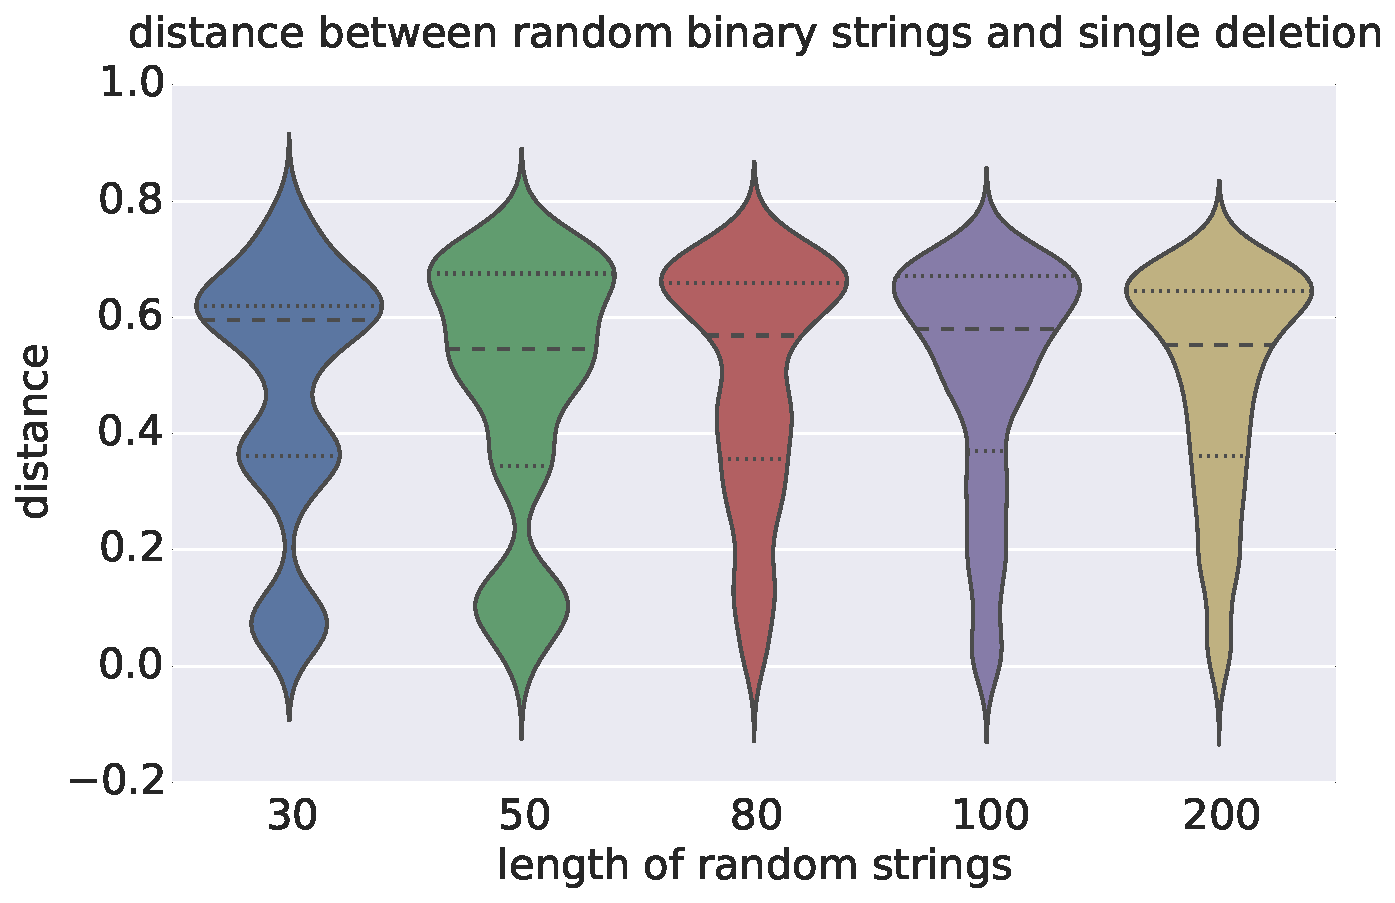
\includegraphics[width=\WDT]{Figures/s1d}};
\node[anchor=west] (B) at (A.east) {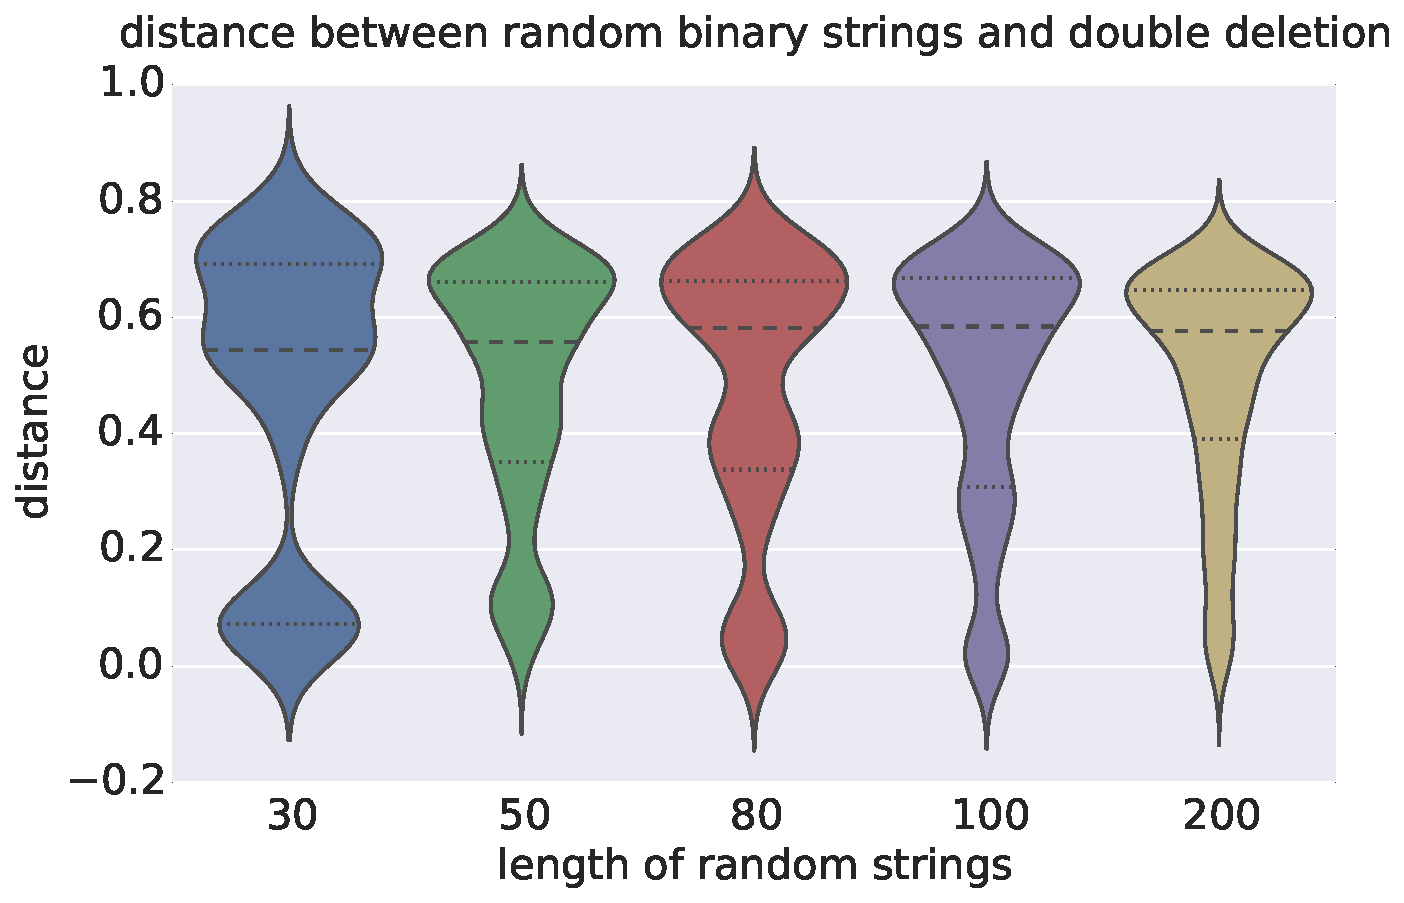
\includegraphics[width=\WDT]{Figures/s2d}};

\node [anchor=north west] at (A.north west) {A};
\node [anchor=north west] at (B.north west) {B};

\node[anchor=north west] (C) at (A.south west) {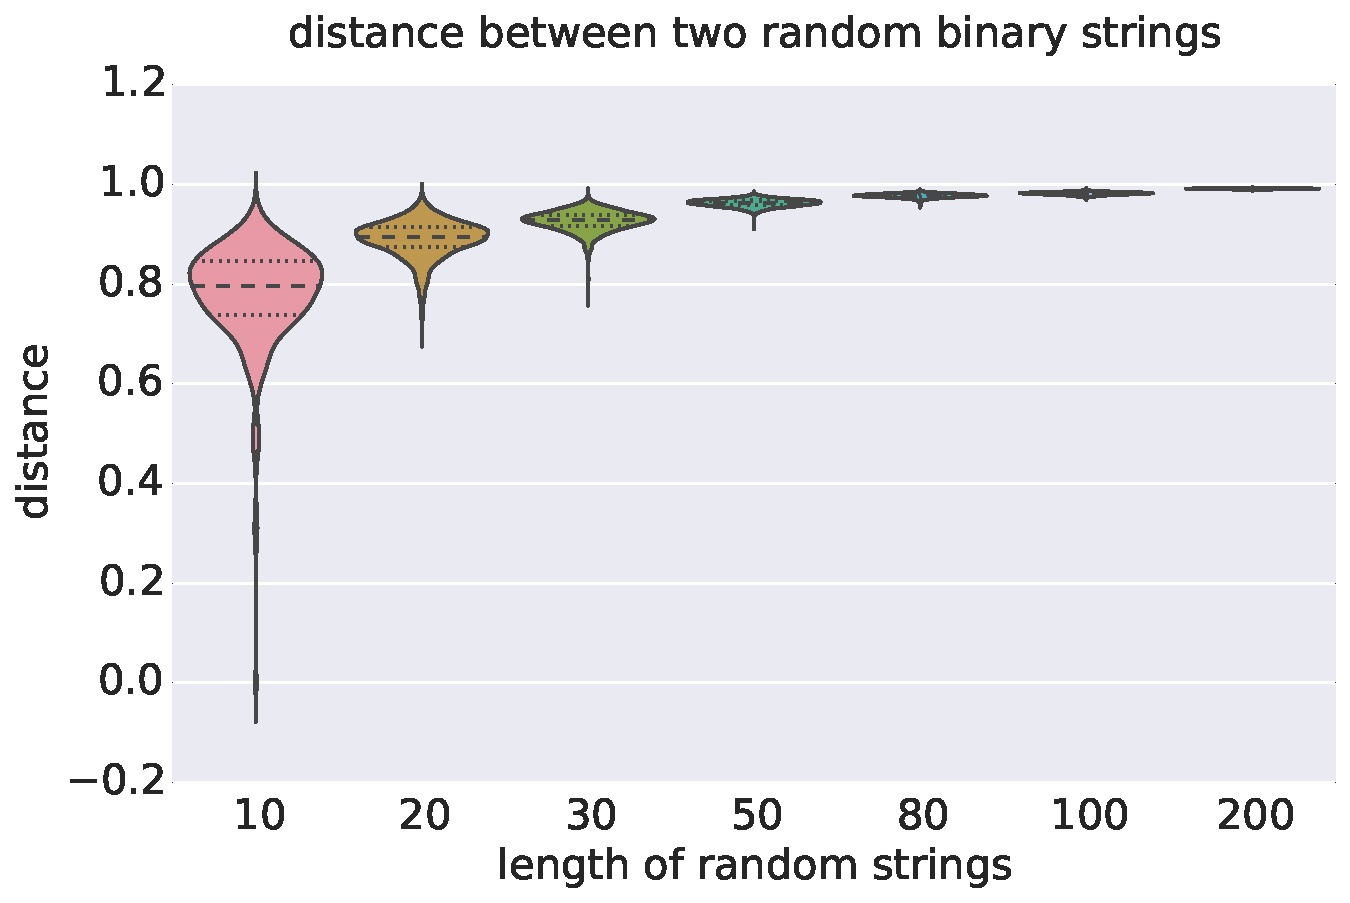
\includegraphics[width=\WDT]{Figures/s3d}};
\node[anchor=west] (D) at ([yshift=-.0in,xshift=.0in]C.east) {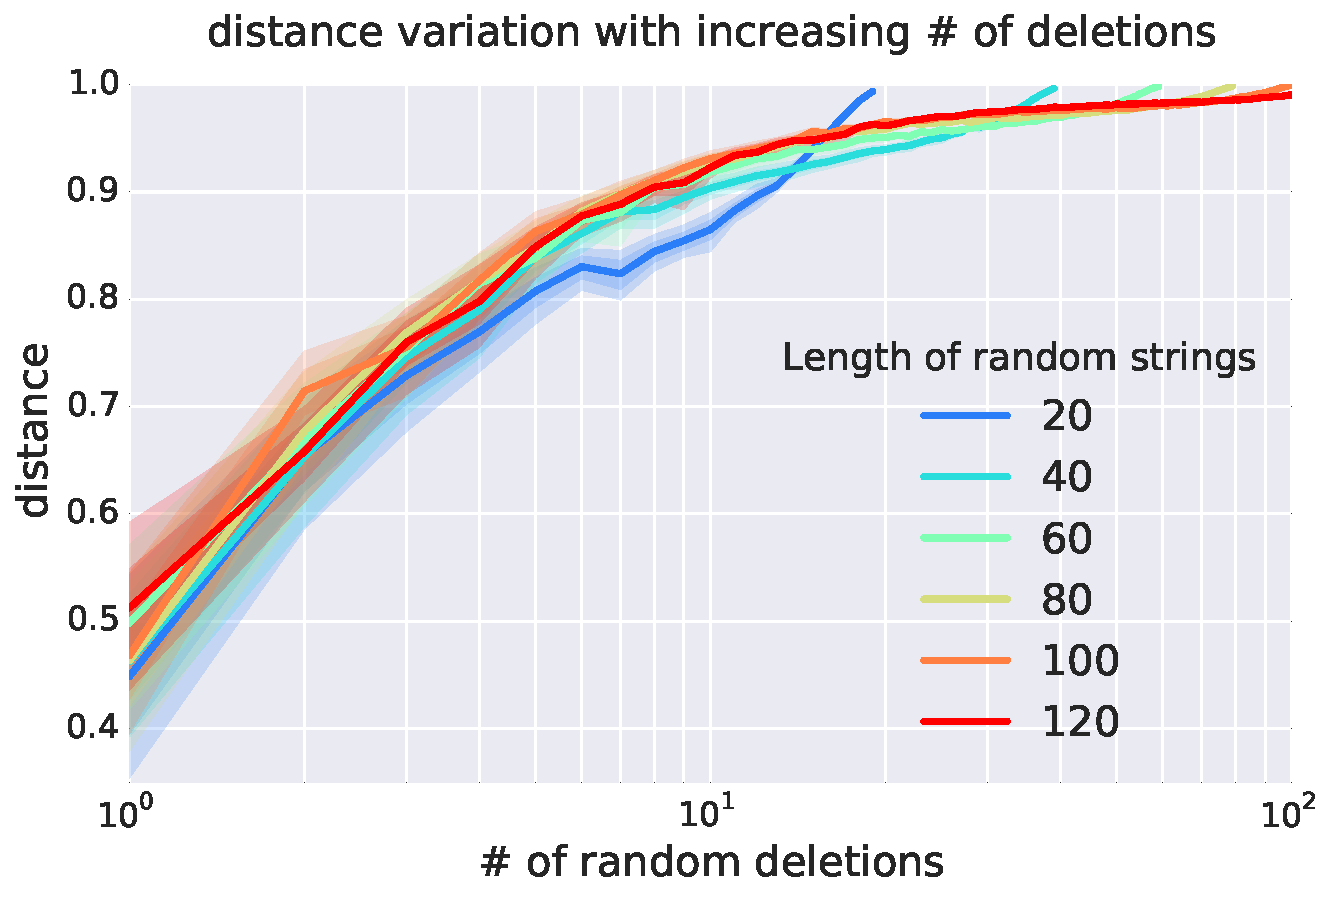
\includegraphics[width=\WDT]{Figures/s4d}};
\node [anchor=north west] at ([yshift=.1in]D.north west) {D};
\node [anchor=north west] at ([yshift=.1in]C.north west) {C};

\end{tikzpicture}
 
\captionN{Effect of deletions/variations on the sequential Jaccard distance between random binary strings. Plate A shows the effect of single deletions on random binary strings of increasing length. Plate B illustrates the same effect for two random deletions. Plate C shows how the distance between two random strings converge to $1$ as the length of the strings is increased. Plate D illustrates the effect of increasing the number of deletions on random binary strings of increasing length, with $99.9999999\%$ confidence bounds. Note that the sequential \textit{weighted} Jaccard distance is more complicated.}
\end{figure*}
%################################
%################################
%%%%%
%
\begin{notn} 
%
\begin{enumerate}
\item The set of disease phenotypes referenced in our database of consideration is denoted as $\D$. We augment $\D$ with an additional symbol $\{d_0\}$ which indicates a ``healthy'' status.
\item The time interval of interest is indexed by  the set of positive integers $\T$, where:
\cgather{
\T = \{ 1, 2, \cdots \}
}
For example, if the unit of time  is chosen to be [\textrm{years}], then a disease reported at $t=1$ refers to the report occurring before the first birthday of the subject.
\item A indexed phenotype is  a tuple:
\cgather{(t,d), t \in \T, d\in \D}
 where the particular reported phenotype is indexed at the age it is reported.
\end{enumerate}
\end{notn}
%
\begin{defn}[History]
A history $h_t$ is a sequence of indexed phenotypes representing the reported medical history of a subject, ending at time index $t$:
\cgather{
h_{t_n} = \left \{(t_1,d_1) ,\cdots , (t_i,d_i),\cdots  , (t_n,d_{n}) \right \}, \notag \\ \textrm{where } t_i \in \T, d_i \in \D, t_1 \leqq \cdots \leqq t_n
}
\end{defn}
\begin{notn}
\begin{itemize}
\item 
For history $h_t$, we denote:
\cgather{
h_t(t_1) = \left \{ \begin{array}{ll}
d \in \D , & \textrm{if } (t_1,d) \in h_t \\
d_0, & \textrm{otherwise}
\end{array}\right.
}
\item Sub-histories are denoted as follows:
\cgather{
h_t\vert_\tau = \{(t',d') \in h_t : t' \leqq \tau \}
}
We also simply write  $h_\tau$ for $h_t \vert_\tau$ where no confusion arises.
\item Also, we use  $\T(h_t)$  to denote the set of timestamps in $h_t$.
\cgathers{
\T(h_t) \subseteqq \T, \textrm{ such that } t' \in \T(h_t) \Rightarrow \exists d \in \D ( \exists (t',d) \in h_t)
}
\end{itemize}
\end{notn}
\begin{notn}
If two appropriately defined empirical distributions $f,g$ pass the Kolmogorov-Smirnov two sample equality test at significance level $\alpha$, then we write:
\cgather{
f \sim_{\KS(\alpha)} g
} 
\end{notn}
%
%\section{Medical Database To Predictive Diagnosis}
\section{Conceptual Framework: The House Function $\Psi$}
%
\begin{notn}[$\epsilon$-Neighborhood of History]
We would define a quasi-metric on the space of histories in the sequel. Open $\epsilon$-neighborhoods in this space, centered at $h_t$, is denoted by  $\big [ h_{t} \big ]_{\epsilon}$
\end{notn}
%
For the purpose of the next definition, we interpret $\big [ h_{t} \big ]_{\epsilon}$ with respect to an arbitrary  quasi-metric on the space of histories. Later, we would make precise the specific metric we use. 
%
\begin{defn}[The House Function $\Psi$]\label{defHouse}
The House function specifies the probability of reporting a specific phenotype at a specific time, conditioned on an $\epsilon$-neighborhood of a specific history:
\cgather[6pt]{
\forall t \in \T, d \in \D,\ \Psi_{\epsilon}(t,d,h_{t-1}) = Pr \left ( (t,d) \big \rvert \big [ h_{t-1} \big ]_{\epsilon}  \right )
}
where, denoting the chosen quasi-metric as $\Theta(\cdot,\cdot)$, we have:
\cgather{
h'_{t'} \in \big [ h_{t-1} \big ]_{\epsilon} \textrm{ if } \Theta(h'_{t'},h_t) < \epsilon
}
\end{defn}

% \noindent\tikz{\node[fill=lightgray!30,inner sep=5pt,]{
% \mnp{0.95\columnwidth}{
The central objective in this work is to efficiently compute the House function, along with estimates of statistical significance.
% }
% };}

The unconditional probability of observing a specific history can now be written in terms of the House function as follows:
\cgather{\label{eq13}
Pr(h_t) = \prod_{i=1}^t \Psi_{\epsilon}(i,h_t(i),h_{i-1})
}
Importantly, there are no Markovian assumptions injected in Eq.~\eqref{eq13}; we do not yet have any notion of state, and the probability of future observations is allowed to depend on the entire observed past. 

The House function  thus represents a model of the 
emergent dynamical relationships in the database, that is maximally agnostic of prior knowledge. The need for conditioning on $\epsilon$-neighborhoods should be clear: even with a substantially large database of patient histories, there are very few exact repeats; implying that probabilities cannot be reliably estimated unless we put togther a large enough set from ``similar'' histories. Also, note that such a notion of similarity must be specified a priori; we cannot for example define histories to be similar if future evolution is close in some sense, since then we would need to quantify what we mean by similar futures (thus we cannot invoke the notion of ``causal states''~\cite{CL12g} directly). The absence of a Markovian assumption at this level makes the framework significantly  more general compared to n-gram models (we do not a priori decide on a bound on $n$). Furthermore, while the formulation definitely is remniscent of a \textit{language model}, note that the presence of substantial repeats of words and phrases in any natural language makes the explicit use of neighborhoods in probability calculations somewhat unnecessary, and rare sequences are generally handled via some kind of  pre-defined smoothing function. In contrast, in our case, almost all histories are rare.

It is clear that we need to explicitly specify the quasi-metric to compute the House function. However, any intutively satisfactory notion of distance that we come up with, must in turn  depend on the probabilistic structure emergent in the space of observed histories, and therefore must functionally depend on the House function itself. This leads to a recursive relationship between the two.

Before proceeding, we note that the average hazard rate  of any phenotype may be expressed in terms of the House function as follows:
%
\cgather{
\forall d \in \D, \zeta(d) = \frac{1}{\T}\sum_{t\in \T} \lim_{\epsilon \rightarrow \infty} \Psi(t,d,[h_t]_\epsilon)
}
%

\begin{notn}
Let $\Psi_\epsilon(t,\cdot,h_{t-1})$ denote a probability distribution over $\D$, such that:
\cgather{
\forall j \in \D, \Psi_\epsilon(t,\cdot,h_{t-1}) \big \vert_j = \Psi_\epsilon(t,j,h_{t-1})
}
\end{notn}

%
\section{The Quasi-Metric $\Theta$}
The quasi-metric is what injects our physical intuition into the problem. Defining a distance between tuple-sequences is not terribly difficult; however identifying a distance function that comports with our physical intuition on the properties that such a function should have, is somewhat more non-trivial.

\subsection{Intuitive Properties Of the Quasi-metric}
\begin{enumerate}
\item Histories which have high unconditional probability of occurrence should be close. In other words, a sequence of common occurrences should not contribute to a large deviation in the computed distance.
\item Rare events should induce  large deviations; if two histories are nearly identical except that one carries the record of an uncommon disease phenotype, then the distance between the two should be large.
 \item  If two histories are substantially different, but share the record of a  rare phenotype, then they should be close under the proposed metric.
\item Permutations of the records in time  should matter. If one history is simply a permutation of another, and such a transformation leads to a reduction in its unconditional probability of occurrence, $i.e.$, makes it more rare, then the distance between them should increase. Even if the unconditional probability is identical, the distance should not be zero.
\item Any distance that we propose must be informed by the database of histories; it must not be computable from the sequences alone in the absence of a  sufficiently large set of observed histories. In other words, classical string edit metrics will not suffice.
\end{enumerate}
Additionally, we should also strive to keep our proposed function as simple as possible. 
%
\begin{defn}[Quasi-metric]\label{defmetric}
Let $h_t,h_{t'}'$ be two histories. Let  $\zeta^{-1}:\D \rightarrow \mathbb{N}
$ be:
\cgather{
\forall d \in \D, t \in \T,  \zeta^{-1}((t,d)) = \left \lceil \frac{1}{\zeta(d)} \right \rceil^\gamma, \gamma > 1, \gamma \in \mathbb{N}
 \intertext{and where:}
\forall d \in \D, \zeta(d) = \frac{1}{\T}\sum_{t\in \T} \lim_{\epsilon \rightarrow \infty} \Psi(t,d,[h_t]_\epsilon)
}
%
Then, we specify the quasi-metric, as a function of $\gamma$, as:
\cgather{
\Theta_\gamma(h_t,h'_{t'}) = \frac{1}{2} \left ( \frac{1}{Pr(h'_{t'})}+ \frac{1}{Pr(h_t)} -2 \right )\J_{\zeta^{-1}}(h_t,h'_{t'})
}
%
Unless otherwise specified, we drop the subscript in $\Theta_\gamma$, and   assume $\gamma=2$ in the sequel. The interpretation of this parameter will be discussed later.
\end{defn}
%
It is immediate from Definition~\ref{defmetric} that $\Theta_\gamma(h_t,h'_{t'})$ is symmetric,  always non-negative, and zero if and only if the histories $h_t,h'_{t'}$ are identical. In particular, we have the following result.
\begin{lem}[Quasi-metric]
If the unconditional probability of the histories is bounded between $(\theta, 1-\theta), \theta > 0$, then $ \Theta_\gamma$ is a $\left (\frac{1}{\theta^2}+O(\theta)\right )$-quasi-metric on the space of histories, for all $ \gamma \in \mathbb{N}$. 
\end{lem}
\begin{IEEEproof}
To be given in SI.
\end{IEEEproof}
%
%It is clear that  $\Theta$ is completely specified by the House function. 
We first explore the salient properties of this quasi-metric, to check that it does indeed satisfy the intuitive constraints laid out before.
\subsection{$\Theta$ Properties}
Let $h_t,h'_{t'}$ be two histories. Then:
\begin{enumerate}
\item If $Pr(h_t) \rightarrow 1, Pr(h'_{t'}) \rightarrow 1$, then clearly they do not contain any rare phenotype, implying that $\J_{\zeta^{-1}}(h_t,h'_{t'})$ remains bounded. It follows that
\cgather{ \frac{1}{Pr(h'_{t'})}+ \frac{1}{Pr(h_t)} \rightarrow 2^+ \Rightarrow \Theta_\gamma(h_t,h'_{t'}) \rightarrow 0^+
}
\item On the other hand, if $Pr(h_t) \rightarrow 0, Pr(h'_{t'}) \rightarrow 0$, but there are no common rare phenotypes, then again $\J_{\zeta^{-1}}(h_t,h'_{t'})$ remains bounded. It then  follows that  $\Theta_\gamma(h_t,h'_{t'}) \rightarrow \infty$.
\item But, if $Pr(h_t) \rightarrow 0, Pr(h'_{t'}) \rightarrow 0$, and the histories share the record of a rare phenotype $d'$ (possibly at different time points), such that $\zeta(d') \rightarrow 0$, then for $\gamma > 1$, the Jaccard term goes to zero faster, and we have $\Theta_\gamma(h_t,h'_{t'}) \rightarrow 0$.
\item Clearly, permutations lead to a positive deviation, since we use the Jaccard distance on the  weighted subword set of the histories (See Definition~\ref{defwsj})
\item It follows from definition that the proposed quasi-metric is informed by the observations in the database, Indeed, as observed before,  $\Theta_\gamma(h_t,h'_{t'})$ may be written exclusively in terms of the House function.
\end{enumerate} 
\section{Computation of the House Function}

\subsection{Recursive Computation}
%
The House function is approximated via the empirical estimate:
\cgather{
\forall d \in \D, \Psi_\epsilon(t,d,h_{t-1}) \approx {\absB{[h_{t-1}]_\epsilon }}^{-1}\sum_{\mathclap{\mspace{50mu}h'_t: h'_{t-1} \in [h_{t-1}]_\epsilon}} \mathbb{I} ((t,d)\in h'_t)
}
where $\mathbb{I} (\cdot )$ is the indicator function. 
Definitions~\ref{defHouse} and \ref{defmetric} might seem to have a circular dependence. To resolve this, one must adopt a recursive approach for computing the House function. Note that at age of $1$ week (assuming our time unit is \textit{weeks}) the past history is empty, and the House function  simply specifies the  unconditional probabilities of the different phenotypes occurring at age $1$ week :
\cgather{
\forall d \in \D, \Psi_{\epsilon}(1,d,h_0)= Pr((1,d) \lvert \varnothing) = Pr((1,d))
}
For computing $\Psi_\epsilon$ at later times, we must first compute $\epsilon$-neighborhoods of histories for the preceding time unit. Since we can compute the House function at age $1$ week, we can compute the distance between histories upto age $1$ week, which then allows us to compute the House functions for age $2$ weeks, which in turn allows us to compute distances between histories upto age 2, and so on.

%  We have the following result.

% \begin{lem}[Computational Complexity]
% Assuming that the total number of phenotypes is significantly smaller than the total number of individual histories (the database size), the asymptotic complexity of computing the House function is linear in the database size.
% \end{lem}

% \subsection{Asymptotic Computational Complexity}
% %
% To do. 
% %
% ##############################
% ##############################
% ##############################
\begin{figure}
\centering
\tikzexternaldisable

\tikzstyle{reverseclip}=[insert path={(current page.north east) --
  (current page.south east) --
  (current page.south west) --
  (current page.north west) --
  (current page.north east)}
]
\def\SCALE{.77}
\begin{tikzpicture}[remember picture,scale=\SCALE,font=\bf\sffamily\fontsize{10}{10}\selectfont]

\begin{scope}
\draw[rotate around={45:(0,0)},fill=SeaGreen1, opacity=.5,  thick, , draw=Green1] (0,0) ellipse (1 and 2);
\draw[name path=ellipse1,rotate around={45:(0,0)},fill=Orchid1,
% pattern=crosshatch,
opacity=.75,  thick, , draw=Orchid4] (0,0) ellipse (.5 and 1);
\draw[name path=line R,opacity=0] (0,0) -- (-.5,1);
\begin{pgfinterruptboundingbox}
\clip[rotate around={45:(0,0)}] (0,0) ellipse (1 and 2) [reverseclip];
 \draw [very thick,black] (-2,-2) to[out=0,in=135] (-1,-1.5) to[out=-45,in=160] (0,0)  ;
\draw [very  thick, black] (-2,-3) to[out=0,in=135] (0,-2.5) to[out=-45,in=200] (0.6,-1)  ;
\draw [very thick, black] (-3,-1) to[out=-20,in=135] (-2,1) to[out=-45,in=220] (-1,1.25)  ;

\end{pgfinterruptboundingbox}
\end{scope}

\begin{scope}
\clip[rotate around={45:(0,0)}] (0,0) ellipse (1 and 2);
\draw [thin, dashed] (-2,-2) to[out=0,in=135] (-1,-1.5) to[out=-45,in=160] (0,0)  ;
\draw [thin, dashed] (-2,-3) to[out=0,in=135] (0,-2.5) to[out=-45,in=200] (0.6,-1)  ;
\draw [thin, dashed] (-3,-1) to[out=-20,in=135] (-2,1)  to[out=-45,in=220] (-1,1.25)  ;
\end{scope}

\node [] at (-1,-1) {$h_t$};
\node [] at (-2,-.5) {$h''_t$};
\node [] at (-.2,-2) {$h_t'$};
\node [circle,fill=white,inner sep=1.1pt] at (-3,-1) {};
\node [circle,fill=white,inner sep=1.1pt] at (-2,-3) {};

\node [circle,fill=gray,inner sep=1.1pt] at (0,0) {};
\node [circle,fill=gray,inner sep=1.1pt] at (.6,-1) {};
\node [circle,fill=gray,inner sep=1.1pt] at (-1,1.25) {};
\draw [line width = 1mm,->,>=stealth,Orchid4,opacity=.8,text opacity=1] (0,0) -- (3.5,.9) node [above,right,pos=1,text opacity=1] {$\Psi_{\epsilon'}(t,\cdot,  h_{t-1})$};
\draw [line width = 1mm,->,>=stealth,opacity=.6,SeaGreen4,,text opacity=1] (0,0) -- (2.5,2) node [above,right,pos=1,text opacity=1] {$\Psi_{\epsilon}(t,\cdot,  h_{t-1})$};
\draw [ thick,->,>=stealth',black,opacity=.7,text opacity=1] (0.6,-1) -- (3.5,-1) node [below,right,pos=1,text opacity=1,text=black] {$Pr((t,\cdot)\vert  h'_{t-1})$};
\draw [ thick,->,>=stealth',black,opacity=.7] (-1,1.25) -- (-.5,2.5) node [below,right,pos=1,text opacity=1,text=black] {$Pr((t,\cdot) \vert  h''_{t-1})$};

\draw [->,>=latex,opacity=.6,rotate around={45:(0,0)}] (0,0) -- (0,1) node [midway,above,pos=1,text opacity=1] {$\epsilon'$};

\draw [->,>=latex,opacity=.6,rotate around={45:(0,0)}] (0,0) -- (.9,.9) node [midway,right,pos=1,text opacity=1] {$\epsilon$};

\end{tikzpicture}

\captionN{Notion of  stable neighborhoods: There should exist some $\epsilon' <\epsilon$, such that $\Psi_\epsilon(t,d,h_{t-1})$ and $\Psi_{\epsilon'}(t,d,h_{t-1})$ is not  too different.}
\end{figure}
% ##############################
% ##############################
\subsection{Calculation of Statistical Significance}
In the development so far, $\epsilon$ appears as a free parameter. However, a choice of too large an $\epsilon$ makes the neighborhood include histories that do not have comparable  futures. When we choose a small enough neighborhood, the probability distribution of the next events should be invariant over   sub-neighborhoods. This leads us to the notion of stable neighborhoods, and allows us to formulate a notion of optimal choice for the parameter $\epsilon$. 
\begin{defn}[$\alpha$-stable Neighborhoods]
For  $\epsilon' < \epsilon$, let:
\cgather{
\forall d \in \D, p(d) \triangleq {\absB{[h_{t-1}]_\epsilon \setminus [h_{t-1}]_{\epsilon'}}}^{-1}\sum_{\mathclap{\mspace{100mu}h'_t: h'_{t-1} \in [h_{t-1}]_\epsilon \setminus [h_{t-1}]_{\epsilon'}}} \mathbb{I} ((t,d)\in h'_t)
\intertext{Then, $\displaystyle [h_{t-1}]_\epsilon$ is $\alpha$-stable if:}
\exists \epsilon' \in (0,\epsilon), \textrm{ such that } 
p \sim_{\KS(\alpha)} \Psi_{\epsilon'}(t,\cdot,h_{t-1})
}
\end{defn}
\begin{defn}[Optimal Significance Pair]
Let us denote:
\cgather{
\epsilon_\alpha \triangleq \sup_{\epsilon \in (0,\infty) } \left ( \{ \epsilon: [h_t]_\epsilon \textrm{ is $\alpha$-stable } \} \cup \{ 0\}   \right )
}
Then, the optimal significance pair $(\alpha^\star,\epsilon^\star)$ w.r.t  $h_{t}$ is defined as:
\cgather{
\epsilon^\star = \sup_{\alpha \in [0,1]} \epsilon_\alpha \\
\alpha^\star = \inf_{\alpha \in [0,1]} \{ \alpha^2: \epsilon_\alpha \leqq \epsilon^\star  \} 
}
%
\end{defn}
%
The optimal significance pair is unique by definition, and is clearly a function of the chosen metric/quasi-metric. Thus, it  can be used to test how well our quasi-metric performs in  identifying functionally similar histories. 
%
\begin{rem}[Ranking metrics via average optimal significance]If we have the option of choosing between different metrics or quasi-metrics, the average optimal significance achieved over the database may be used to rank the options, and choose the one achieving the higher average optimal value.
\end{rem}
The optimal significance pair dictates the confidence bounds on the House function estimate.
\begin{lem}[Optimal Confidence Bounds] If  $(\alpha^\star,\epsilon^\star)$ is the optimal signifcance pair w.r.t. $h_{t-1}$, then the  confidence bounds at significance level $\alpha^\star$ on $\Psi_{\epsilon^\star}(t,\cdot,h_{t-1})$ is given by:
\cgather{
\forall d \in \D, \Psi_{\epsilon^\star}(t,d,h_{t-1}) \pm \frac{2k'}{\sqrt{\abs{[h_{t-1}]_{\epsilon^\star} }}} \intertext{where we have:}
\K(k')=1-\sqrt{\alpha^\star} \intertext{and $\K$ is the Kolmogorov distribution function:} 
\forall x \in \mathbb{R}, \K(x) = \frac{\sqrt{2\pi}}{x} \sum_{k=1}^\infty e^{-\frac{1}{8} \left ( (2k-1)\frac{\pi}{x}\right )^2}
}
\end{lem}
\begin{IEEEproof}
Since $(\alpha^\star, \epsilon^\star)$ is the optimal significance pair at $h_{t-1}$:
\cgather{
\exists \epsilon' < \epsilon, p \sim_{\KS(\sqrt{\alpha^\star})} \Psi_{\epsilon'}(t,\cdot,h_{t-1})
}
Fix an admissible $\epsilon' < \epsilon$. Let us denote:
\cgather{
\frac{\abs{[h_{t-1}]_{\epsilon'}}}{\abs{[h_{t-1}]_{\epsilon}}}=r \leqq 1
}
Now, from the formulation of the standard KS two sample test:
\cgather{
\norm{p-\Psi_{\epsilon'}(t,\cdot,h_{t-1})}_\infty > \frac{k'}{\sqrt{r(1-r)\abs{[h_{t-1}]_{\epsilon}}}} \textrm{ w.p. } \sqrt{\alpha^\star}
}
Let the true distribution we are attempting to infer is $f$. Then:
\mltlne{\label{eq35}
\norm{p-f}_\infty + \norm{f-\Psi_{\epsilon'}(t,\cdot,h_{t-1})}_\infty \\\geqq  \norm{p-\Psi_{\epsilon'}(t,\cdot,h_{t-1})}_\infty > \frac{k'}{\sqrt{r(1-r)\abs{[h_{t-1}]_{\epsilon}}}} \textrm{ w.p. } \sqrt{\alpha^\star}
}
Now, it is obvious, that we have the mixture:
\cgather{\label{eq36}
\Psi_{\epsilon}(t,\cdot,h_{t-1}) = r \Psi_{\epsilon'}(t,\cdot,h_{t-1}) + (1-r) p
}
Using Eq.~\eqref{eq36}, we get two bounds:
\begin{subequations}
\mltlne{
\norm{\Psi_{\epsilon}(t,\cdot,h_{t-1})- f}_\infty \leqq  \frac{rk'}{\sqrt{r(1-r)\abs{[h_{t-1}]_{\epsilon}}}} \\+ \norm{p-f}_\infty \textrm{ w.p. } 1-\sqrt{\alpha^\star}
}
\mltlne{
\norm{\Psi_{\epsilon}(t,\cdot,h_{t-1})- f}_\infty \leqq  \frac{(1-r)k'}{\sqrt{r(1-r)\abs{[h_{t-1}]_{\epsilon}}}} \\+ \norm{\Psi_{\epsilon'}(t,\cdot,h_{t-1})-f}_\infty \textrm{ w.p. } 1-\sqrt{\alpha^\star}
}
\end{subequations}
We can rewrite the above bounds as:
\begin{subequations}
\mltlne{
\norm{\Psi_{\epsilon}(t,\cdot,h_{t-1})- f}_\infty >  \frac{rk'}{\sqrt{r(1-r)\abs{[h_{t-1}]_{\epsilon}}}} \\+ \norm{p-f}_\infty \textrm{ w.p. } \sqrt{\alpha^\star}
}
\mltlne{
\norm{\Psi_{\epsilon}(t,\cdot,h_{t-1})- f}_\infty >  \frac{(1-r)k'}{\sqrt{r(1-r)\abs{[h_{t-1}]_{\epsilon}}}} \\+ \norm{\Psi_{\epsilon'}(t,\cdot,h_{t-1})-f}_\infty \textrm{ w.p. } \sqrt{\alpha^\star}
}
\end{subequations}
Summing the last two inequalities, we get:
\mltlne{
2\norm{\Psi_{\epsilon}(t,\cdot,h_{t-1})- f}_\infty > \frac{k'}{\sqrt{r(1-r)\abs{[h_{t-1}]_{\epsilon}}}} \\+ \norm{p-f}_\infty + \norm{f-\Psi_{\epsilon'}(t,\cdot,h_{t-1})}_\infty \textrm{ w.p. } \sqrt{\alpha^\star}
}
Using Eq.~\eqref{eq35}, we get:
\mltlne{
2\norm{\Psi_{\epsilon}(t,\cdot,h_{t-1})- f}_\infty >  \frac{2k'}{\sqrt{r(1-r)\abs{[h_{t-1}]_{\epsilon}}}} \textrm{ w.p. } \alpha^\star }
The proof is then completed by noting that the maximum value of $r(1-r)$ is $1/4$.
\end{IEEEproof}
\begin{rem}[The Matching Problem]
Matching refers to finding patient histories which are similar. 
Computation of the House function at least partially  solves the matching problem, since, every history in $[h_t]_{\epsilon^\star}$ is matched to $h_t$. There is however the issue of  demographics stratification, which we have ignored so far. However, this is a trivial issue, easily solved by partitioning the database a priori into demographic strata.
\end{rem}
% ##############################
\begin{figure}
\centering
\tikzexternaldisable

\def\SCALE{.6}
\begin{tikzpicture}[font=\bf\sffamily\fontsize{10}{10}\selectfont,scale=.7]
\node [] (A1) {
\begin{tikzpicture}[scale=\SCALE]
  \draw [ultra thick,IndianRed2] (-2,2) to[out=0,in=135] (-1,1.5) to[out=-45,in=160] (0,0) to[out=0,in=135] (1.5,.5) to[out=-45,in=-135] (2.5,0)to[out=45,in=-180] (3.5,.5) ;
  \def\x{-.3}
  \draw [ultra thick,DodgerBlue4!80] (-2,-2) to[out=0,in=135] (-1,-1.55+\x) to[out=-45,in=160] (0,0.1+\x) to[out=0,in=135] (1.5,.57+\x) to[out=-45,in=-135] (2.45,0+\x)to[out=45,in=-180] (3.5,.4+\x) ;
%
\node [] at (-1.3,-1.3) {$h'_t$};
\node [] at (-1.3,1.3) {$h_t$};
\draw [thin, lightgray] (0,-2) -- (0,2) node [pos=0,below,text=black] {$t_1$};
\draw [thin, lightgray] (1,-2) -- (1,2) node [pos=0,below,text=black] {$t_2$};
\draw [thin, lightgray] (2,-2) -- (2,2) node [pos=0,below,text=black] {$t_3$};
\draw [->,>=stealth',ultra thick, gray] (-3,-3) -- (3,-3) node [midway,below,text=black] {time};
%
\draw[fill=Green3,fill opacity=.25,  thick, , draw=black] (0,0) ellipse (.2 and .5);
\draw[fill=gray,fill opacity=.25,  thick, , draw=black] (1,0.4) ellipse (.2 and .5);
\draw[fill=gray,fill opacity=.25,  thick, , draw=black] (2,-.1) ellipse (.2 and .5);
%
\node [] at (-2.5,0) {\LARGE A};
\end{tikzpicture}};
\node [anchor=west] at (A1.east) {
\begin{tikzpicture}[scale=\SCALE]
  \draw [ultra thick,IndianRed2] (-2,2) to[out=0,in=135] (-1,1.5) to[out=-45,in=160] (0,0) to[out=0,in=135] (1.5,.95) to[out=-45,in=-135] (2.5,1.2)to[out=45,in=-180] (3.5,.75) ;
  \def\x{-.3}
  \draw [ultra thick,DodgerBlue4!80] (-2,-2) to[out=0,in=135] (-1,-1.55+\x) to[out=-45,in=160] (0,0.1+\x) to[out=0,in=135] (1.5,-.57+\x) to[out=-45,in=-135] (2.45,-1+\x)to[out=45,in=-180] (3.5,-1.4+\x) ;
%
\node [] at (-1.7,-1.3) {$h'_t$};
\node [] at (-1.7,1.2) {$h_t$};
\draw [thin, lightgray] (0,-2) -- (0,2) node [pos=0,below,text=black] {$t_1$};
\draw [thin, lightgray] (1,-2) -- (1,2) node [pos=0,below,text=black] {$t_2$};
\draw [thin, lightgray] (2,-2) -- (2,2) node [pos=0,below,text=black] {$t_3$};
%
\draw[fill=Green3,fill opacity=.25,  thick, , draw=black] (0,0) ellipse (.2 and .5);
% \draw[fill=gray,fill opacity=.25,  thick, , draw=black] (1,0.4) ellipse (.2 and .5);
% \draw[fill=gray,fill opacity=.25,  thick, , draw=black] (2,-.1) ellipse (.2 and .5);
%
\draw [->,>=stealth',ultra thick, gray] (-3,-3) -- (3,-3) node [midway,below,text=black] {time};
\node [] at (-2.5,0) {\LARGE B};
\end{tikzpicture}};
\end{tikzpicture}

\captionN{Notion of  causal states. Plate A illustrates the situation $h_t \sim h'_t$. Unlike plate  B, here the histories remain close in future, inducing the notion that $h_t,h'_t$ lead to a common causal state at time $t$.}\label{figcausal}
\end{figure}
% ##############################
\section{Inducing The Notion of Causal States}
We define a right invariant equivalence relation on the space of histories to induce the notion of states.
\begin{defn}[Causal States]\label{defcausal}
Two histories $h_t,h'_t$ are equivalent (denoted as $h_t \sim h'_t$) if,
\cgather{
\forall z = \{(t+1,d_1), \cdots, (t+i,d_i), \cdots, (t+m,d_m)  \}, d_i \in D, \notag \\
\forall d \in D, \Psi_{\epsilon}(t+m+1,d,h_t\cup z) = \Psi_{\epsilon}(t+m+1,d,h'_t\cup z)
}
\end{defn}
It follows from Defn.~\ref{defcausal} that:
\cgather{
h_t \sim h'_t \Rightarrow  h_t\cup z \sim h'_t \cup z
}
for any right extension $z$ into future. The property of right invariant equivalence is what 
formalizes the notion of a dynamical state: once we arrive at a state, the future behavior 
no longer distinguishes between different paths that brought us there. 
% \subsection{Optimizing Metric Resolution $\epsilon$}

%\begin{figure*}
%\end{figure*} 

}%%%ENDALLOWDISPLAYBREAKS

\begin{figure*}[b]
\centering

\tikz{\node[ path fading=fade out, fill=lightgray,inner sep=20pt]{

\includegraphics[width=2in]{Figures/house1}};}

\end{figure*}


\bibliographystyle{siam}
\bibliography{BibLib1,eqref}

% %\centering
% \clearpage


\end{document}
